\documentclass[crop,tikz]{standalone}
\usepackage{tikz}
\usetikzlibrary{calc}
\usetikzlibrary{positioning}
\begin{document}
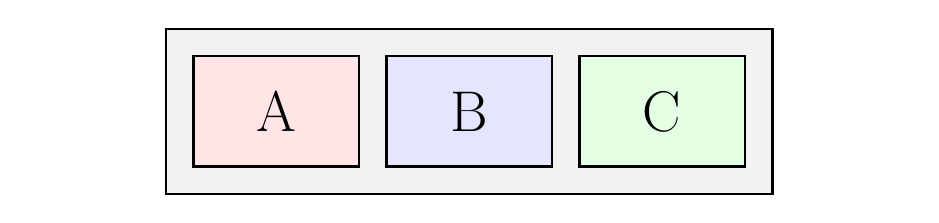
\begin{tikzpicture}[scale=0.07,rotate=0]
	
	%Background
	\draw[draw=white, fill=white] (0,0) rectangle (160,30);
		
	%Frame
	\draw[thick, draw=black, fill=gray!10] (25,0) rectangle (135,30);

	%Segments
	%A
	\draw[thick, draw=black, fill=red!10] (30,5) rectangle (60,25);
	\node at (45,15) {\huge A};

	%B
	\draw[thick, draw=black, fill=blue!10] (65,5) rectangle (95,25);
	\node at (80,15) {\huge B};
	
	%C
	\draw[thick, draw=black, fill=green!10] (100,5) rectangle (130,25);
	\node at (115,15) {\huge C};
	

	
\end{tikzpicture}
\end{document}